% ------------------------------------------------------------------
%  Figura: Objetivos (slide 8) — 3 tarjetas + métricas compactas abajo
% ------------------------------------------------------------------
\documentclass[tikz, border=0.2cm]{standalone}
\usepackage[utf8]{inputenc}
\usepackage[T1]{fontenc}
\usepackage{libertine}
\usepackage{amssymb}
\usepackage{xcolor}

\definecolor{primary}{HTML}{280091}
\definecolor{secondary}{HTML}{4C5CC5}
\definecolor{accent}{HTML}{3FCFD5}
\definecolor{exgreen}{HTML}{00B299}
\definecolor{alertred}{HTML}{C0392B}

\begin{document}
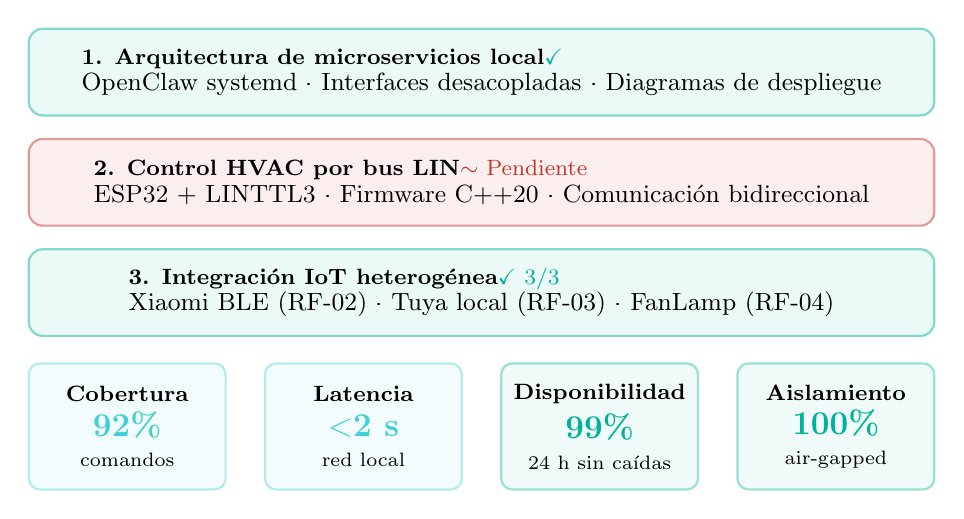
\begin{tikzpicture}[
  card/.style={draw=#1!50, fill=#1!8, rounded corners=5pt,
               minimum width=11.5cm, minimum height=1.1cm, align=left,
               font=\footnotesize, line width=0.8pt},
  stat/.style={draw=#1!40, fill=#1!6, rounded corners=4pt,
               minimum width=2.5cm, minimum height=1.6cm, align=center,
               font=\footnotesize, line width=0.8pt},
]

% --- Objetivo 1 ---
\node[card=exgreen] at (0, 2.5) {
  \textbf{1. Arquitectura de microservicios local}\hfill\textcolor{exgreen}{\checkmark}
  \\ {\small OpenClaw systemd · Interfaces desacopladas · Diagramas de despliegue}
};

% --- Objetivo 2 ---
\node[card=alertred] at (0, 1.1) {
  \textbf{2. Control HVAC por bus LIN}\hfill\textcolor{alertred}{$\sim$ Pendiente}
  \\ {\small ESP32 + LINTTL3 · Firmware C++20 · Comunicación bidireccional}
};

% --- Objetivo 3 ---
\node[card=exgreen] at (0, -0.3) {
  \textbf{3. Integración IoT heterogénea}\hfill\textcolor{exgreen}{\checkmark\ 3/3}
  \\ {\small Xiaomi BLE (RF-02) · Tuya local (RF-03) · FanLamp (RF-04)}
};

% --- Métricas compactas ---
\node[stat=accent]   at (-4.5, -2.0) {\textbf{Cobertura}\\[0.1cm]{\large\color{accent}\textbf{92\%}}\\[0.05cm]{\scriptsize comandos}};
\node[stat=accent]   at (-1.5, -2.0) {\textbf{Latencia}\\[0.1cm]{\large\color{accent}\textbf{$<$2 s}}\\[0.05cm]{\scriptsize red local}};
\node[stat=exgreen]  at (1.5, -2.0)  {\textbf{Disponibilidad}\\[0.1cm]{\large\color{exgreen}\textbf{99\%}}\\[0.05cm]{\scriptsize 24 h sin caídas}};
\node[stat=exgreen]  at (4.5, -2.0)  {\textbf{Aislamiento}\\[0.1cm]{\large\color{exgreen}\textbf{100\%}}\\[0.05cm]{\scriptsize air-gapped}};

\end{tikzpicture}
\end{document}
